\documentclass[a4paper,english,12pt]{article}
\usepackage{%
	amsfonts,%
	amsmath,%	
	amssymb,%
	amsthm,%
	algorithm,%
	babel,%
	bbm,%
	etex,%
	%biblatex,%
	caption,%
	centernot,%
	color,%
	dsfont,%
	enumerate,%
	epsfig,%
	epstopdf,%
	geometry,%
	graphicx,%
	hyperref,%
	latexsym,%
	mathtools,%
	multicol,%
	pgf,%
	pgfplots,%
	pgfplotstable,%
	pgfpages,%
	proof,%
	psfrag,%
	subfigure,%	
	tikz,%
	ulem,%
	url%
}	
\usepackage[noend]{algpseudocode}
\usepackage[mathscr]{eucal}
\usepgflibrary{shapes}
\usetikzlibrary{%
  	arrows,%
	backgrounds,%
	chains,%
	decorations.pathmorphing,% /pgf/decoration/random steps | erste Graphik
	decorations.text,%
	matrix,%
  	positioning,% wg. " of "
  	fit,%
	patterns,%
  	petri,%
	plotmarks,%
  	scopes,%
	shadows,%
  	shapes.misc,% wg. rounded rectangle
  	shapes.arrows,%
	shapes.callouts,%
  	shapes%
}

\theoremstyle{plain}
\newtheorem{thm}{Theorem}[section]
\newtheorem{lem}[thm]{Lemma}
\newtheorem{prop}[thm]{Proposition}
\newtheorem{cor}[thm]{Corollary}

\theoremstyle{definition}
\newtheorem{defn}[thm]{Definition}
\newtheorem{conj}[thm]{Conjecture}
\newtheorem{exmp}[thm]{Example}
\newtheorem{assum}[thm]{Assumptions}
\newtheorem{axiom}[thm]{Axiom}

\theoremstyle{remark}
\newtheorem{rem}{Remark}
\newtheorem{note}{Note}
\newtheorem{fact}{Fact}

\newcommand{\norm}[1]{\left\lVert#1\right\rVert}
\newcommand{\indep}{\!\perp\!\!\!\perp}
\DeclarePairedDelimiter\abs{\lvert}{\rvert}%
\newcommand\numberthis{\addtocounter{equation}{1}\tag{\theequation}}
\newcommand{\tr}{\operatorname{tr}}
\newcommand{\R}{\mathbb{R}}
\newcommand{\N}{\mathbb{N}}
\newcommand{\E}{\mathbb{E}}
\newcommand{\Z}{\mathbb{Z}}
\newcommand{\B}{\mathscr{B}}
\newcommand{\C}{\mathcal{C}}
\newcommand{\T}{\mathscr{T}}
\newcommand{\F}{\mathcal{F}}
\newcommand{\G}{\mathcal{G}}
%\newcommand{\ba}{\begin{align*}}
%\newcommand{\ea}{\end{align*}}
\DeclareMathOperator*{\argmax}{arg\,max}
\renewcommand{\qedsymbol}{$\blacksquare$}
\makeatletter
\def\BState{\State\hskip-\ALG@thistlm}
\makeatother

\makeatletter
\def\th@plain{%
  \thm@notefont{}% same as heading font
  \itshape % body font
}
\def\th@definition{%
  \thm@notefont{}% same as heading font
  \normalfont % body font
}
\makeatother
\date{}

%opening
\title{Lecture 3: Minimax \& Neyman Pearson Hypothesis Testing}
\author{}

\begin{document}
\maketitle
In this lecture we complete the theoretical portion of our discussion of Minimax hypothesis testing rule and begin with the Neyman-Pearson hypothesis testing approach.

\section{Minimax Hypothesis Testing (Cotd. from Lecture 2)}
We have already looked at the Minimax Hypothesis testing approach when the function $V(x)$ is continuous at the point of the maxima. This is not always so in several problems of interest. We therefore consider the case when $V$ has an interior maximum (i.e. maxima lies between $\pi_{L} \in [0,1]$) but the derivative does not exist at this point. Since the derivative is not unique, there is a concern as to which decision rule $\delta_{\pi_{L}}$ should be chosen.

We begin by defining two decision rules as limits to the maxima from the right and left, 
\begin{eqnarray}
&\delta_{\pi_{L}}^{-}& = \underset{\pi_0 \uparrow \pi_L}{lim} \delta_{\pi_0} = \underset{\pi_0 \uparrow \pi_L}{lim} \mathbbm{1}_{\{L(y) > \tau (\pi_0)\}}, \nonumber \\
&\delta_{\pi_{L}}^{+}& = \underset{\pi_0 \downarrow \pi_L}{lim} \delta_{\pi_0},
\end{eqnarray}
where, $\delta_{\pi_0}$ is the indicator function corresponding to the likelihood function being greater than the threshold. For $\delta_{\pi_{L}}^{-}$ the critical region $\Gamma_{1}^{-}$ and for $\delta_{\pi_{L}}^{+}$ the critical region $\Gamma_{1}^{+}$ is given by,
\begin{eqnarray}
\Gamma_{1}^{-} = \underset{\pi_0 \uparrow \pi_L}{\bigcap} \{ L(y) \geq \tau(\pi_0)\} = \{ y \in \Gamma | L(y) \geq \tau (\pi_L) \} \nonumber \\
\Gamma_{1}^{+} = \underset{\pi_0 \downarrow \pi_L}{\bigcup} \{ L(y) > \tau(\pi_0)\} = \{ y \in \Gamma | L(y) > \tau (\pi_L) \}.
\end{eqnarray}
Let us now consider a Bayesian decision rule $\tilde{\delta_{\pi_L}}$ that uses $\Gamma_1^{-}$ with probability $q$ (where $q \in [0,1]$) and $\Gamma_1^{+}$ with probability $1-q$, at the point $L(y) = \tau$. We are basically implying that we know the optimum decision rule at all other points except at the point of discontinuity, at which we now choose between the limiting decision rules by the throw of a biased coin. Therefore,
\begin{equation}
\tilde{\delta_{\pi_L}}  = 
\begin{cases}
choose~ H_1 &if~y \in \Gamma_1^{+}\\
choose~ H_0 &if~y \in {(\Gamma_1^{-})}^c\\
choose~ H_1 ~w.p.~ q &if~y~ is~ on~ boundary~ of~ \Gamma_1^{-}.
\end{cases}
\end{equation}
Since conditional risk depends on the boundary condition, we write it as,
\begin{equation}
R_j(\tilde{\delta_{\pi_L}}) = qR_j(\delta_{\pi_L}^{-}) + (1-q)R_j(\delta_{\pi_L}^{+}),~~j=[0,1], 
\end{equation}
which is nothing but,
\begin{eqnarray}
R_0(\tilde{\delta_{\pi_L}}) = qR_0(\delta_{\pi_L}^{-}) + (1-q)R_0(\delta_{\pi_L}^{+}) \nonumber \\
R_1(\tilde{\delta_{\pi_L}}) = qR_1(\delta_{\pi_L}^{-}) + (1-q)R_1(\delta_{\pi_L}^{+}). 
\end{eqnarray}
So for the minimax rule at equality,
\begin{equation}
max\{ R_0(\tilde{\delta_{\pi_L}}), R_1(\tilde{\delta_{\pi_L}}) \} = R_0(\tilde{\delta_{\pi_L}}) = R_1(\tilde{\delta_{\pi_L}})
\end{equation}
Therefore, the conditional risk equations for equality condition are,
\begin{equation*}
qR_0(\delta_{\pi_L}^{-}) + (1-q)R_0(\delta_{\pi_L}^{+}) = qR_1(\delta_{\pi_L}^{-}) + (1-q)R_1(\delta_{\pi_L}^{+}).
\end{equation*}
\begin{equation*}
q\{R_0(\delta_{\pi_L}^{-}) - R_0(\delta_{\pi_L}^{+})\} + R_0(\delta_{\pi_L}^{+}) = q\{R_1(\delta_{\pi_L}^{-}) - R_1(\delta_{\pi_L}^{+})\} + R_1(\delta_{\pi_L}^{+})
\end{equation*}
\begin{equation}
R_0(\delta_{\pi_L}^{+}) - R_1(\delta_{\pi_L}^{+}) = q\{R_0(\delta_{\pi_L}^{+}) - R_1(\delta_{\pi_L}^{+}) + R_1(\delta_{\pi_L}^{-}) - R_0(\delta_{\pi_L}^{-})\}.
\end{equation}
So,
\begin{equation}
\label{qeq}
q = \frac{R_0(\delta_{\pi_L}^{+}) - R_1(\delta_{\pi_L}^{+})}{R_0(\delta_{\pi_L}^{+}) - R_1(\delta_{\pi_L}^{+}) + R_1(\delta_{\pi_L}^{-}) - R_0(\delta_{\pi_L}^{-})}
\end{equation}
This gives us the probability with which we choose the alternate hypothesis at the boundary. We now represent the unconditional risk by $V$. Since $V$ is concave, it must have left hand and right hand derivative at $\pi_L$, which is denoted by $V^{'}(\pi_L^{-})$ and $V^{'}(\pi_L^{+})$. Now,
\begin{eqnarray}
V^{'}(\pi_L^{-}) &=& \frac{d}{d \pi_0} r(\pi_0 , \delta_{\pi_L^{-}}) \nonumber \\
&=& \frac{d}{d\pi_0}\{\pi_0 R_0(\delta_{pi_L^{-}}) + (1-\pi_0)R_1(\delta_{\pi_L^{-}}) \} \nonumber \\
&=& R_0(\delta_{\pi_L^{-}}) - R_1(\delta_{\pi_L^{-}}) 
\end{eqnarray}
Similarly, $V^{'}(\pi_L^{+}) = R_0(\delta_{\pi_L^{+}}) - R_1(\delta_{\pi_L^{+}})$. Hence equation \ref{qeq} can be written as
\begin{equation}
q = \frac{V^{'}(\pi_L^{+})}{V^{'}(\pi_L^{+}) - V^{'}(\pi_L^{-})}
\end{equation}
We can analyse the importance of the above equation in the following manner. Figure \ref{fig:AWGN} shows the case in which  V is discontinuous at the point of maxima. The decision rule here is $\tilde{\delta_{\pi_L}}$. By varying the probability q from 0 to 1 different slopes of the line $r(\pi_0, \tilde{\delta_{\pi_L}})$ can be obtained. The particular value of q obtained from the equation above gives rise to the horizontal line.   
\begin{figure}[h]
\centering
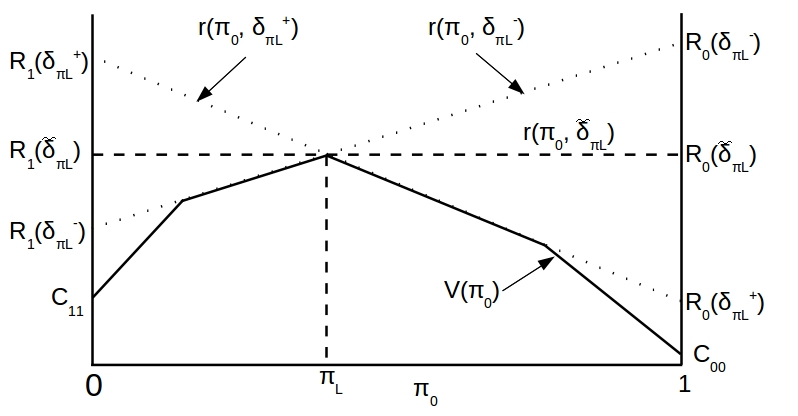
\includegraphics[width=0.7\linewidth]{Figures/Lec3_Fig1.jpg}
\caption[rdr]{Action of the randomized decision rule}
\label{fig:AWGN}
\end{figure}
\section{Neyman-Pearson Hypothesis Testing}
Earlier we saw two different methods, Bayesian and Minimax, for hypothesis testing. It can be noticed that in both cases the predominant assumption is \textit{uniform cost}, i.e. there is a penalty of detecting $H_0$ when $H_1$ is true and vice-versa but no penalty for not detecting an event. This is not a desirable feature - if for instance, the hypothesis detection corresponds to detection of enemy aircraft by a RADAR system. In that case we would rather allow for slightly higher false detection (detecting an aircraft when none exists) to ensure higher probability of detection. It will be shown in this section that the Neyman Pearson criteria actually achieves this goal.
We begin by defining the required terminology.
\begin{defn}
In hypothesis testing, an error is defined as \textit{Type-I Error or False Alarm} when the hypothesis $H_1$ is detected given $H_0$ is true and \textit{Type-II Error or Missed Detection} when the hypothesis $H_0$ is detected given $H_1$ is true. The correct acceptance of $H_1$ is termed as \textbf{Detection}. 
\end{defn}
\begin{defn}
The probability of Type-II Error is termed as the probability of miss or miss probability, denoted by $P_M (\delta)$. Thus, the probability of detection is $P_D(\delta) = 1 - P_M(\delta)$. 
\end{defn}
\begin{defn}
The probability of Type-I Error is termed as the probability of false alarm, denoted by $P_F (\delta)$. 
\end{defn}
\begin{defn}
The randomized decision rule $\tilde{\delta}: \Gamma \rightarrow [0,1]$ is a function for $H_0$ versus $H_1$ with the interpretation that for $y \in \Gamma$, $\tilde{\delta}$ is the conditional probability with which we accept $H_1$ given that we observe $Y=y$. 
\end{defn}
For a randomized rule $\tilde{\delta}$ the probability of false alarm is given by, 
\begin{equation}
P_F(\tilde{\delta}) = E_0\{\tilde{\delta}(Y)\} = \int_{\Gamma} \tilde{\delta}(y) p_0(y) \mu (dy),
\end{equation} 
where, $E_0$ is the expectation under hypothesis $H_0$. Similarly, detection probability of a randomized detection rule $\tilde{\delta}$ is given by,
\begin{equation}
P_D(\tilde{\delta}) = E_1\{\tilde{\delta}(Y)\} = \int_{\Gamma} \tilde{\delta}(y) p_1(y) \mu (dy),
\end{equation} 
where, $E_1$ is the expectation under hypothesis $H_1$.

\subsection{Neyman-Pearson Criterion}
The Neyman-Pearson criterion is based on constrained optimization problem in which the probability of detection is maximized subject to probability of false alarm within a limit. Mathematically, the criterion is given by -
\begin{equation}
\underset{\delta}{max}~~P_{D} (\delta)~~ subject~ to~ P_F(\delta) \le \alpha,
\end{equation}
where $\alpha$ is the sufficiency level of the test. We will now state and prove the Neyman-Pearson lemma.
\begin{lem}{The Neyman-Pearson Lemma}
Let $\alpha > 0$, 
\begin{itemize}
\item[i] \texttt{Optimality} Let $\tilde{\delta}$ be any decision rule satisfying $P_F(\tilde{\delta}) \le \alpha$ and let $\tilde{\delta^{'}}$ be any other decision rule of the form:
\begin{equation}
\label{decrule}
\tilde{\delta^{'}} (y) = 
\begin{cases}
1 &if~p_{1}(y) > \eta p_0 (y) \Rightarrow L(y) > \eta\\
\gamma(y) &if~L(y) = \eta\\
0 &if~L(y) < \eta,
\end{cases}
\end{equation}
where, $\eta \geq 0$ and $0 \leq \gamma(y) \leq 1$ such that $P_F(\tilde{\delta}) = \alpha$, then, $P_D(\tilde{\delta^{'}}) \geq P_D(\delta^{'})$.
\item[ii] \texttt{Existence} For every $\alpha \in (0,1)$ there is a decision rule $\tilde{\delta}_{NP}$ of the form \ref{decrule} with $P(y) = \gamma_0$ (a constant), for which $P_F(\tilde{\delta}_{NP}) = \alpha$
\item[iii] \texttt{Uniqueness} Let $\delta^{''}$, i.e. any $\alpha$-level Neyman-Pearson decision rule for $H_0$ versus $H_1$. Then $\delta^{''}$ must be of the form \ref{decrule} except possibly on a subset of $\Gamma$ having zero probability under $H_0$ and $H_1$.
\end{itemize}
\begin{proof}{}
[i] We define the decision rule in the usual manner-
\begin{equation}
[\tilde{\delta}^{'} (y) - \tilde{\delta} (y) ][p_1(y) - \eta p_0(y)] \geq 0 ~~~~ \forall y\in \Gamma.
\end{equation}
Thus,
\begin{equation}
\int_{\Gamma} [\tilde{\delta}^{'} (y) - \tilde{\delta} (y) ][p_1(y) - \eta p_0(y)]  \mu (dy) \geq 0, 
\end{equation}
\begin{eqnarray}
\int_{\Gamma} \tilde{\delta}^{'} (y) p_1(y)  \mu (dy) &-& \int_{\Gamma} \eta \tilde{\delta}^{'} (y) p_0(y)  \mu (dy) \nonumber \\
- \int_{\Gamma} \tilde{\delta} (y) p_1(y)  \mu (dy) &+& \int_{\Gamma} \eta \tilde{\delta} (y) p_0(y)  \mu (dy) \geq 0,
\end{eqnarray}
\begin{eqnarray}
\int_{\Gamma} \tilde{\delta}^{'} (y) p_1(y)  \mu (dy) &-& \int_{\Gamma} \tilde{\delta} (y) p_1(y)  \mu (dy) \nonumber \\
\geq  \int_{\Gamma} \eta \tilde{\delta}^{'} (y) p_0(y)  \mu (dy)  &-& \int_{\Gamma} \eta \tilde{\delta} (y) p_0(y)  \mu (dy).
\end{eqnarray}
But we know that, 
\begin{equation}
P_D(\tilde{\delta}) = \int_{\Gamma} \tilde{\delta}(y) p_1(y) \mu (dy) ~~ \& ~~  P_F(\tilde{\delta}) = \int_{\Gamma} \tilde{\delta}(y) p_0(y) \mu (dy).
\end{equation}
Therefore, we can write the above equation as,
\begin{eqnarray}
\label{faineq}
P_D(\tilde{\delta}^{'}) - P_D(\tilde{\delta}) & \geq &  \eta [P_F(\tilde{\delta}^{'}) - P_F(\tilde{\delta})] \nonumber \\
& \geq & \eta (\alpha - P_F(\tilde{\delta})) ~~~~~ \because P_F(\tilde{\delta}^{'})  = \alpha \nonumber \\
& \geq & 0 ~~~~~~~~~~~~~~~~~~~~~ \because P_F(\tilde{\delta})  \leq \alpha.
\end{eqnarray}
Hence,
\begin{equation}
P_D(\tilde{\delta}^{'}) \geq P_D(\tilde{\delta}).
\end{equation}
[ii] Let $\eta_0$ be the smallest number such that 
\begin{equation}
\eta_0 = inf\{\eta \in \mathbb{R}_{+} : (P_0 \{L(y)\} > \eta) \leq \alpha\}.
\end{equation}
The term $(P_0 \{L(y)\} > \eta)$ is indicative of CCDF-like form which exhibits right continuity. Now, if $P_0{L(y) > \eta_0} < \alpha $, then choose,
\begin{eqnarray}
\gamma_0 &=& \frac{\alpha - P_0(p_1(y) > \eta_0 p_0(y))}{P_0(p_1(y) = \eta_0 p_0(y))} \nonumber \\
&=& \frac{\alpha - P_0(L(y) > \eta)}{P_0(L(y) > \eta_0)},
\end{eqnarray}
otherwise, choose $\gamma_0$ arbitrarily. Then, on defining $\tilde{\delta_{NP}}$ to be the decision rule of form \ref{decrule}, with $\eta = \eta_0$ and $\gamma(y) = \gamma_0$, we have, 
\begin{eqnarray}
P_F(\tilde{\delta_{NP}}) &=& E_0\{\tilde{\delta_{NP}}(Y)\}  \nonumber \\
&=& P_0(p_1(Y) > \eta_0 p_0(Y)) + \gamma_0 P_0(p_1(Y) = \eta_0 p_0(Y)) \nonumber \\
&=& \alpha.
\end{eqnarray}
Thus, we have chosen a decision rule of the form \ref{decrule} with $\gamma(y)$ constant and false-alarm probability $\alpha$. 

[iii] Let $\tilde{\delta^{'}}$ be of the form \ref{decrule} and $\tilde{\delta^{''}}$ be any other $\alpha$-level Neyman-Pearson decision rule, then,
\begin{equation}
P_D(\tilde{\delta^{''}}) = P_D(\tilde{\delta^{'}})
\end{equation}
and therefore, by equation \ref{faineq},
\begin{eqnarray}
0 &\geq & \alpha - P_F(\tilde{\delta^{''}}) \nonumber \\
&\geq & 0 ~~~~~ (from~ part~ i). 
\end{eqnarray}
Hence, $P_F(\tilde{\delta^{''}}) = \alpha$. We know that,
\begin{eqnarray}
&\int_{\Gamma}& [\tilde{\delta}^{'} (y) - \tilde{\delta} (y) ][p_1(y) - \eta p_0(y)]  \mu (dy) \geq 0 \nonumber \\ 
&=&\{ P_D(\tilde{\delta^{'}}) - P_D(\tilde{\delta^{''}})\} - \eta \{ P_F(\tilde{\delta^{'}}) - P_F(\tilde{\delta^{''}})\} \nonumber \\
&=& 0.
\end{eqnarray}
Since the integrand is non-negative it implies that it is zero except possibly on a set of zero probability under $H_0$ and $H_1$. Thus $\tilde{\delta^{'}}$ and $\tilde{\delta^{''}}$ differ only on the set of where $L(y) = \eta$ and hence both have the same form \ref{decrule} possibly differing only in choice of $\gamma(y)$.
\end{proof}
\end{lem}

\end{document}